% Preamble
% --------
\documentclass[12pt]{article}

\newcommand{\codename}[0]{\texttt{apex-sim}~}

% Packages
% --------
\usepackage{blindtext} %for boilerplate text (\blindtext)
\usepackage{geometry} %for paper dimensions and margins
\usepackage{graphicx} % for including graphics
\usepackage{hyperref} % for hyperlink support
\usepackage{todonotes}

% Page Setup
% ----------
\geometry{letterpaper, margin=1in}

% Title content and formatting
% ----------------------------
\title{Apex Instruction Set Architecture Simulator (\texttt{apex-sim}) \\ Phase 2 Documentation}
\author{Matthew Cole \\ \texttt{mcole8@binghamton.edu}
\and
Brian Gracin \\ \texttt{bgracin1@binghamton.edu}}
\date{19 November 2016}

\begin{document}
% Emit title content
% ------------------
\pagenumbering{gobble}
\maketitle
\tableofcontents
\newpage
\listoffigures
\listoftables
\newpage
\pagenumbering{arabic}

%---------------

\section{Design}
\codename is a simulator for the \textit{Architecture Pipeline EXample} (APEX) Instruction Set Architecture (ISA).
\codename consists of the following components:
\begin{itemize}
  \item \texttt{main.cpp} contains the driver program. The driver program provides file input for instructions, user interface operations, maintaining persistent simulator state and statistics monitoring. This component is discussed in section \ref{sec:driver}.
  \item \texttt{apex.cpp} contains helper functions for \texttt{main.cpp}. These include wrapper functions that delegate interface actions down to individual classes.
  \item Several source files provide the objects modeling components of the pipeline. These components are discussed in section \ref{sec:classes}. Briefly, they are
	\begin{itemize}
		\item \texttt{code.cpp} models the simulator's read-only instructions file.
		\item \texttt{cpu.cpp} (plus its associated helper functions in \texttt{simulate.cpp}) models the stages in the pipeline and interact with the Instruction Queue (IQ) and Reorder Buffer (ROB). It is responsible for overall execution of a single cycle through its helper function \texttt{simulate}. 
		\item \texttt{data.cpp} models the simulator's read-write main memory.
		\item \texttt{iq.cpp} models the simulator's IQ.
		\item \texttt{registers.cpp} models the simulator's unified register file.
		\item \texttt{stage.cpp} models a single stage in the pipeline. It also doubles as an inflight instruction or entry in the IQ or ROB. This allows advancement of an inflight instruction to be greatly simplified.
	\end{itemize}
	\item \texttt{simulate.cpp} provides the functions that allow the CPU to simulate working on each of its stages, inter-stage communication through advancement, stalls for basic inter-stage interlocks, out-of-order execution and reordering, and forwarding. These implementation details are described in section \ref{sec:implementation}.
\end{itemize}
Figure \ref{fig:overview} shows class interactions and data flow between each of the stages and support classes.
Finally, we discuss our team's work log in section \ref{sec:worklog}.

\begin{figure}
  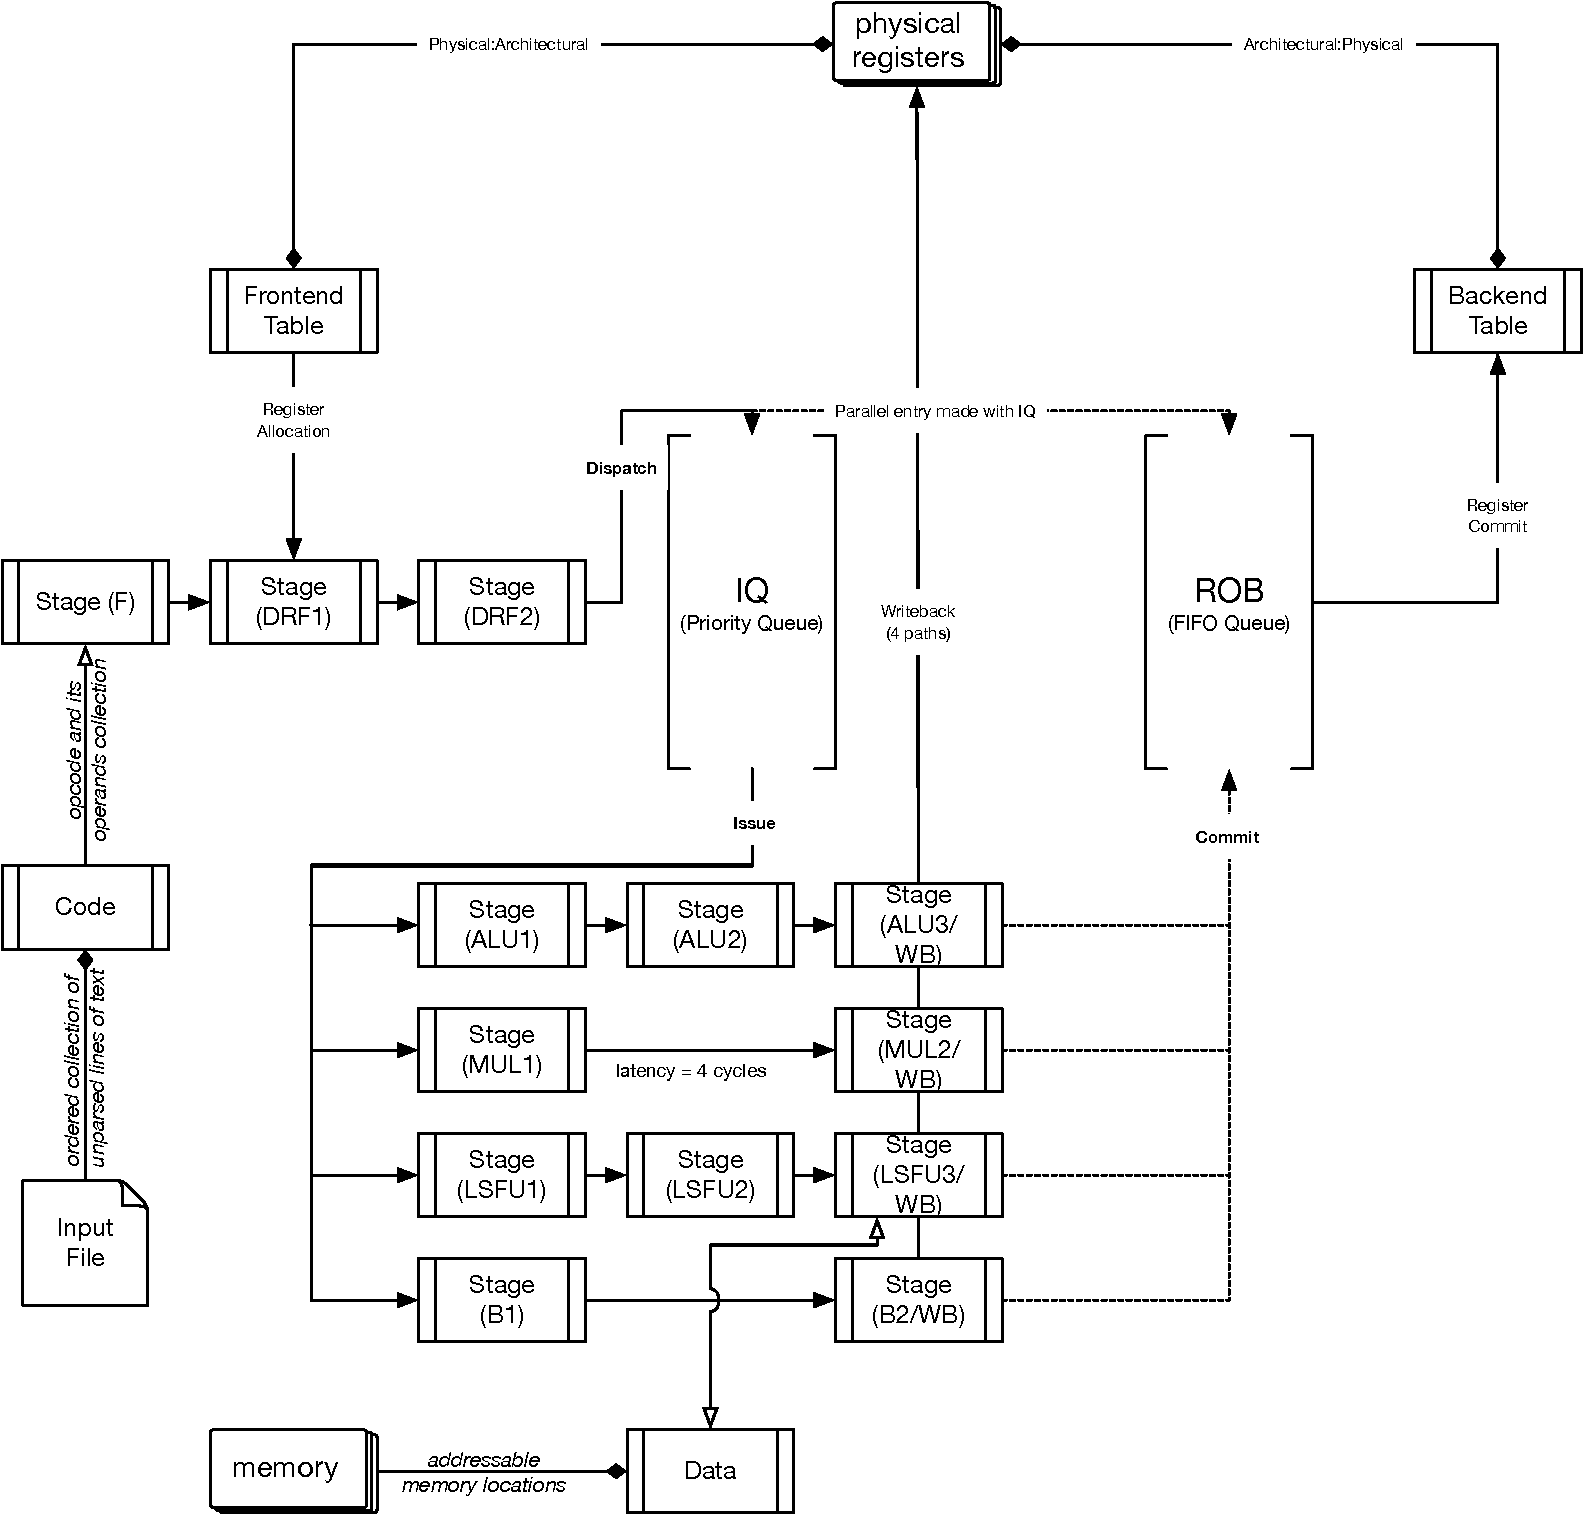
\includegraphics[width=\linewidth]{./figs/apex-sim-overview-2.pdf}
  \caption{APEX pipeline and class data flows.}
  \label{fig:overview}
\end{figure}

\subsection{Driver Program}
\label{sec:driver}
The \codename entry point file is \texttt{main.cpp}. Besides maintaining simulator state variables for the current cycle, program counter and instructions filename, this program shepherds execution through the lifecycle of the program and provides a user interface for interacting with the simulator. The functionality of the driver program is as follows:
\begin{enumerate}
  \item Verify sanity of command line inputs (lines 23-32).
  \item Instantiate class instances for the simulator (lines 34-40).
  \item Perform the initialization of each pipeline stage (line 43).
  \item Prepare and begin the simulator user interface's operations (lines 48-54).
  \item Parse user interface inputs and delegate actions to interface helper functions (lines 57-127).
\end{enumerate}

\texttt{main.cpp} also provides helper functions which delegate work down to class instances in \texttt{apex.cpp}. These functions are:
\begin{itemize}
  \item \texttt{help()} displays the user interface keyboard shortcuts. It's invoked at startup, on request from the user, and whenever the user provides an input which is not recognized.
  \item \texttt{initialize()} resets the simulator state, and invokes the class instances' own \texttt{\textit{classname}.initialize()} functions which reset the instances' internal state.
  \item \texttt{display()} displays the simulator internal state variables as well as delegated calls to each class' \texttt{\textit{classname}.display()} function.
  \item \texttt{stats()} displays simulator execution statistics.
  \item \texttt{simulate()} is the most important of the helper functions. It is responsible for controlling simulation of the \texttt{CPU.simulate()} function for a given number of cycles, and allowing the CPU class to communicate that it has encountered an error, reached EOF of a code file without a HALT instruction, or has processed a HALT instruction through the pipeline.
  \item \texttt{quit()} gracefully halts the simulator and triggers a final call to \texttt{display()}.
\end{itemize}

\subsection{Classes}
\label{sec:classes}
\codename models each major component of the APEX system as a standalone class. Unless mentioned below, these classes did not change appreciably from release v1.0 and are not discussed further in this report. Please see the release v1.0 documentation for discussion of these unchanged classes.

\subsubsection{Issue Queue}
\label{sec:iq}
\codename's issue queue (IQ) uses C++11's Standard Template Library (STL) deque container to model a priority queue. 
Each entry in the deque is a Stage class instance. 
This allows inflight instructions to seamlessly dispatch from the DRF2 stage into the IQ, and issue out into one of the function units. 
Entries are inherently sorted by timestamp of fetching, ensuring that removing entries with earlier program-ordered are preferentially removed before later program-ordered instructions if both are ready. 
Additionally, this mechanism allows us to determine if an later \texttt{LOAD} instruction is attempting to bypass an earlier \texttt{STORE} instruction and prevent its issue. 
The use of the deque container was precipitated by the queue container not having a standard iterator.

\subsubsection{Reorder Buffer}
\label{sec:rob}
The reorder buffer (ROB) likewise uses a deque container for the same design reasons as the IQ, however it is a strict FIFO queue. 
This allows instructions which may have been issued out-of-program order to be committed in-program order. 
Whenever an entry is made in the IQ, a parallel entry is made and queued in the ROB. 
This ensures that the head of the ROB always points to the earliest dispatched instruction. 
Each of the function units' (FU) writeback (WB) stage contents are compared by opcode and timestamp to the ROB head once they become ready. 
When a match occurs, this allows that FU to commit its contents to the back-end register file and de-queue the ROB entry. 
In the case of the LSFU, it also allows memory access to occur.
This enforces memory in-order execution.

\subsubsection{Registers}
The Registers class retains its basic structure as a register file, using an STL::map whose key is a register "tag" (a string), and whose value is a two-tuple of value (an integer) and validity (a bool).
However, in phase two, we added three components.
First, a front-end rename table mapping physical register tag to architectural register tag (STL::map).
Second, a back-end rename table mapping architectural register tag to physical register tag (STL::map).
Third, a free list (STL::vector), listing free physical registers, sorted by their tag's integral value.
This assures that the lowest numbered physical register is preferentially allocated. Section \ref{sec:allocation} discusses this further.

\subsubsection{CPU and Stages}
The functionality and design of the Stage class is largely unchanged from phase 1. 
However, the CPU's structure changed dramatically from phase 1.
\begin{itemize}
  \item DRF stage was split into two stages.
  \item MUL FU was split from the larger ALU FU.
  \item MEM stage was replaced by a LSFU.
  \item WB stage was replaced by a specialized WB stage for each FU
\end{itemize}
Figure \ref{fig:overview} shows the interactions between these new classes.

%-----------------------
\section{Implementation}
\label{sec:implementation}
In this section, we will discuss key aspects of our simulator's execution: the stage-wise reverse-ordered execution, register renaming, dispatch, issue, commit, register value forwarding.

\subsection{Reverse-Ordered Execution}
When we say \textit{reverse-ordered execution}, what we mean is that the \texttt{simulate()} function generally proceeds in what appears to be the opposite order of the pipeline flow. 
That is, later stages in the pipeline perform their tasks in any given phase before earlier stages, and the Branch FU performs its work before the other function units. 
This scheme prevents runaway by an inflight instruction or crossing up values between stages.
This function is broken up into four phases, each providing one general task of the overall cycle's worth of simulation. 

\subsubsection{Forwarding}
Stages attempt to forward. 
Table \ref{tab:fwdscenarios} describes scenarios where \codename performs forwarding from later stages to earlier stages in order to reduce bubbles caused by waiting for flow dependencies to resolve. 
In \codename this is accomplished in \texttt{simulate.cpp} during the forwarding phase (lines \todo{Add forwarding code's line numbers}). 
The instructions' source sets and destination sets are enumerated in table \ref{tab:instsets}.

\begin{table}
  \centering
  \caption{APEX Forwarding Scenarios}
  \label{tab:fwdscenarios}
  \begin{tabular}{l|l|p{5.0in}}
    From & To & Description\\
    \hline
    B2 & B1 & Occurs when B2 has a \texttt{BAL} instruction, and B1 has the X register in its source set. \\
    B2 & IQ & Occurs when B2 has a \texttt{BAL} instruction, and one or more IQ entries is a \texttt{BAL} or \texttt{JUMP} with the X register in its source set. \\
    \hline
    ALU3 & IQ & Occurs when ALU3's destination set has a union with an IQ entry's source set. \\
    ALU3 & ALU2 & Occurs when ALU3's destination set has a union with ALU2's source set. \\
    ALU3 & MUL1 & Occurs when ALU3's destination set has a union with MUL1's source set. \\
    \hline
    ALU2 & ALU1 & Occurs when ALU2's destination set has a union with ALU1's source set.\\
    ALU2 & MUL1 & Occurs when ALU2's destination set has a union with MUL1's source set.\\
    ALU2 & B1 & B1's opcode is \texttt{BAL} or \texttt{JUMP}, ALU2's destination set has a union with B1's source set. \\
    ALU2 & LSFU2 & LSFU2's opcode is \texttt{LOAD} or \texttt{STORE}, ALU2's destination set has a union with LSFU2's source set. \\
    ALU2 & LSFU1 & LSFU2's opcode is \texttt{LOAD} or \texttt{STORE}, ALU2's destination set has a union with LSFU1's source set. \\
    ALU2 & IQ & ALU2's destination set has a union with an IQ entry's source set. \\
    \hline
    MUL2 & IQ & MUL2's destination set has a union with an IQ entry's source set. \\
    \hline
    MUL1 & ALU1 & MUL1's destination set has a union with ALU1's source set. \\
    MUL1 & B1 & B1's opcode is \texttt{BAL} or \texttt{JUMP} and MUL1's destination set has a union with B1's source set. \\
    MUL1 & LSFU2 & MUL1's destination set has a union with LSFU2's source set. \\
    MUL1 & LSFU1 & MUL1's destination set has a union with LSFU1's source set. \\
    MUL1 & IQ & MUL1's destination set has a union with an IQ entry's source set. \\
    \hline
    LSFU3 & LSFU2 & LSFU3's destination set has a union with LSFU2's source set. \\
    LSFU3 & LSFU1 & LSFU3's destination set has a union with LSFU1's source set. \\
    LSFU3 & ALU1 & LSFU3's destination set has a union with ALU1's source set. \\
    LSFU3 & MUL1 & LSFU3's destination set has a union with MUL1's source set. \\
    LSFU3 & LIQ & LSFU3's destination set has a union with an entry in the IQ's source set. \\
  \end{tabular}
\end{table}

\begin{table}
  \centering
  \caption{APEX Instruction Source and Destination Sets}
  \label{tab:instsets}
  \begin{tabular}{l|c|c}
    Instruction & Destination Set Operand Indices & Source Set Operand Indices\\
    \hline
    Arithmetic					 	& 0 & 1,2\\
    MOVC 							& 0 & - \\
    LOAD							& 0 & 1 \\
    STORE							& 1 & 0 \\
    BAL, JUMP						& - & 0 \\
    BZ, BNZ 						& - & - \\
    HALT, NOP						& - & - \\
  \end{tabular}
\end{table}

\subsubsection{Committing}
In this phase, the stages' contents of each of the four WB stages are compared to the ROB's head. If the stage is ready, not empty, and the opcode and timestamp match between stage and ROB head, the instruction is committed.
Committing allows register values to writeback, allows memory access for the LSFU, deallocates registers back into the free list, pops the ROB head, and empties the WB stage.
This phase occurs in lines \todo{add committing source code line numbers}, and takes advantage of the ROB class' \texttt{commit()} function to perform each of the tasks listed above.

\subsubsection{Advancing}
Next, stages other than those which commit are allowed to advance.
Advancing occurs only if the following conditions are all met:
\begin{itemize}
  \item The sending stage is not empty.
  \item The sending stage is ready (i.e. it has completed its work in a previous cycle's working phase).
  \item The receiving stage is empty (i.e. it advanced its contents in this cycle or a previous cycle).
\end{itemize}
Advancing takes advantage of the Stage class' \texttt{advance()} function to perform this logic and to copy contents.
This phase occurs in lines \todo{add advancing phase source code lines}.

\subsubsection{Working}
Then, stages perform their work as one might expect. 
For example, the ALU performs either arithmetic, logical operations or a constant move into a register.
Other stages have their own working phase tasks, and they can be seen in lines \todo{add working phase source code lines}.


\subsection{Register Renaming and Allocation}
\label{sec:renamealloc}

\subsubsection{Allocation}
\label{sec:allocation}
%%%% For Brian 

\subsubsection{Renaming}
\label{sec:renaming}
%%%% For Brian

\subsection{Dispatch}
Instructions are dispatched from the DRF2 stage to the IQ using the IQ class' \texttt{dispatchInst(Stage\&)} function when DRF2 is ready and not empty. 
At the same time, an identical entry is added to the ROB using the ROB class' \texttt{addStage(Stage\&)} function. 
There are three exceptions to this flow.
First, if DRF2 contains a \texttt{HALT} instruction, it is not dispatched because keeping the \texttt{HALT} in DRF2 prevents further instructions from entering the IQ (unless a branch instruction flushes DRF2), and because it is part of the halting detection logic.
Second, if DRF2 contains a \texttt{NOP} instruction, it is not dispatched because the instruction is idempotent and belongs to no FU.
Third, if there is already a control flow instruction in the IQ, design limitations given by the specification prevent a second control flow instruction from entering the IQ.
This is checked using the IQ's \texttt{hasEntryWithOpcode(String opcode)} function with each of the control flow instructions. 
Once dispatch occurs, or it is determined that no dispatch can occur, the relevant statistics are updated within the CPU simulation function.

\subsection{Issue}
As noted in section \ref{sec:iq}, the IQ is a priority queue.
This means that we issue from the IQ to a waiting function unit using the IQ's \texttt{issue(...)} function.
This function uses the following logic to select the highest priority entry for issue:
\begin{itemize}
  \item Only ready entries can be issued. This means all operands needed in the first stage of the applicable FU are ready.
  \item The ready entry with the lowest time stamp should be issued first. This is accomplished by selecting the entry closest to the IQ head with the assumption that since entries were added in program order, they remain stored within the container in program order no matter how many dispatch and issue actions occur.
\end{itemize}
Once it is determined that issue occurs or no issue can occur, the relevant statistics are updated within the CPU simulation function.

\subsection{Commit}
Commits occur when inflight instructions reach one of the four WB stages. 
Their opcode and timestamp are compared against the ROB's head to determine which (if any) should commit. 
As noted above, the ROB is a true FIFO queue, even though it is implemented as a dual-ended deque container.
This decision was made in order to permit the use of an iterator to traverse the ROB for flushing.

\subsection{Flushing}
Whenever a branch is taken, entries in the IQ, ROB and any stage must be flushed if its timestamp is \textit{later} than the timestamp of the instruction causing the branch to be taken. 
This is achieved using \texttt{flush()} functions. 
These functions receive an integral value for the timestamp from the instruction generating the flush, and \-- in the case of the IQ and Stage functions \-- a handle to the registers so that they can cause the allocated registers they hold to be deallocated.
For the IQ and ROB's version of the \texttt{flush()} function, an iterator across the collection simplifies the process.

\subsection{Statistics}
As noted above, statistics counters are updated throughout the execution span of the simulator. They are calculated using the \texttt{stats()} function in \texttt{apex.cpp}. 
This will also display the stats to the console either when the \texttt{stats()} or \texttt{display()} functions are called. 


%-------------------
\section{Work Log}
\label{sec:worklog}
We open-sourced \codename under the MIT license, and developed it using a GitHub repository. \footnote{The repository is available at \url{https://github.com/colematt/apex-sim}}
This repository contains this documentation, all source code, reference materials on the APEX ISA semantics, and other related materials.
Additionally, it contains an in-depth look at our work progress over the course of this project at a much finer grain than this report contains.
As of writing this report, \todo{Add number of commits} commits were made with a total of \todo{Add number of lines of code} lines of code.
Naturally, such a volume of code and the required levels of collaboration would have been nearly impossible without the use of some sort of repository.
We encourage the curious reader to see these statistics in depth using the \textbf{Pulse} and \textbf{Graphs} tabs available on the repository.
Brian Gracin was the team lead for this release of the project. He is behind the overall design, register renaming and the overwhelming majority of troubleshooting.
Matthew Cole rebuilt the simulation functions and user interfaces from release version 1.0, and maintained the repository and documentation.


Table \ref{tab:worklog} is a broad, chronological overview of work performed by each member. 

\begin{table}
\centering
\caption{Chronological Work Log}
\label{tab:worklog}
\begin{tabular}{l|p{2.75in}|p{2.75in}}
Date         	& Matthew's Task
				& Brian's Task \\
\hline
Dec 5, 2016  	& Moved source files into their own directory, updated Makefile.
				& Began modifying Registers class to support URF operations. Created Front-end, Back-end table, Free-list. Prototyped API functions to class. \\
Dec 6, 2016  	& Updated UI for new commands specified in Phase 2. Added stats mechanisms. Updated display methods.
				& Further work on Registers class, updated function to create new instances of registers. Began work on ROB class. \\
Dec 7, 2016		& Allowed templating Stages to IQ and ROB deques. Continued work on final report.
				& Completed ROB and IQ class architectures. Added commit and head-compare utility functions to ROB and IQ for programmer convenience. \\
Dec 8, 2016		& Visibility and inter-class communications pathways. Added halting logic.
				& Initial compilation and end-to-end testing. Added issue utility function to IQ for programmer convenience. \\
Dec 9, 2016		& Continued work on documentation.
				& Continued work on documentation.\\
Dec 10, 2016	& Continued work on documentation. Fixed blocking for advance functions. Began work phase code for all FUs.
				& Completed issue, committing and writeback design. Extensive end-to-end troubleshooting.\\
Dec 11, 2016	& Finalized Work phase, Advancing phase and Forwarding phase in \texttt{simulate()} function. Squashed 3 issues.
				& Continued troubleshooting on all classes.\\
Dec 12, 2016	& Completed final report, troubleshooting, screen captures and submission package.
				& Substantial troubleshooting and \textbf{Checkpointed Release v.2.0!}\\
\end{tabular}
\end{table}

%---------------
\newpage
\appendix
\section{Appendix: Screen Captures}
\todo{Add screen captures.}
\end{document}
